\section{Front-End Package}

	The class diagram \ref{fig: Class diagram for the front-end} shows the structure we will use for this package.
	
	\begin{figure}
	\begin{center}
	\includegraphics[bb=25 720 300 830, clip]{figure/class_frontend.ps}%35 540 560 830
	\caption{Class diagram for the front-end}
	\label{fig: Class diagram for the front-end}
	\end{center}
	\end{figure}
	


	\subsection{Component ``enter choice''}
		
		\begin{description}
	
		\item[Identifier~:]EnterChoice
		\item[Type~:]Method
		\item[Function-processing~:]Offer to read data or to run the simulation for the user. Transmits the result to the ``connect'' component.
		\item[Dependencies~:]-
		\item[Interfaces~:]Output : formalisation or simulation
		\item[Data~:]-

		\end{description}
	
	
  	\subsection{Component ``connect depending on choice''}
	
		\begin{description}
	
		\item[Identifier~:]Connect
		\item[Type~:]Method
		\item[Function-processing~:]Launch the read of the data or launch the simulation depending on the choice enter in the ``enterChoice'' component.
		\item[Dependencies~:]The component  ``enterChoice'' must be executed before this component is called.
		\item[Interfaces~:]Take as input the result of ``enterChoice''.
		\item[Data~:]-

		\end{description}

%  	\subsection{Component ``process manually input data''}
%	\begin{description}
%	\item[Identifier~:]ProcessManData
%	\item[Type~:]Module
%	\item[Function-processing~:]Process the data that are entered manually %using the interface. The data entered by the user (generally matrix
%	and function) are converted to a specified format in order to be %transmitted to the model formalisation package.
%	\item[Dependencies~:]The package  ``model formalisation'' must be %executed after this component is called.
%	\item[Interfaces~:]Take as input the data entered by the user.
%	\item[Data~:]-
%	\end{description}
	

	
\section{Model Formalisation Package}
	The class diagram \ref{fig: Class diagram for model formalisation} shows the structure we will use for this package.
	
	\begin{figure}
	\begin{center}
	\includegraphics[scale=0.85, bb=20 500 560 830, clip]{figure/class_formalisation.ps}
	\caption{Class diagram for model formalisation}
	\label{fig: Class diagram for model formalisation}
	\end{center}
	\end{figure}


	\subsection{Component ``fill dynamic system''}	
	
		\begin{description}
	
		\item[Identifier~:]FillDS
		\item[Type~:]Module
		\item[Function-processing~:]Fill the dynamic system part of the \ac{nsds}.
		\item[Dependencies~:]This component can be executed before, after or meanwhile the processing of the ``fill relations'' and the ``fill non smooth law'' component.
		\item[Interfaces~:]Take as input the data given by the Input/Output/Plug-in package. The output is the representation of the dynamic system.
		\item[Data~:]An inherited class of the DynamicSystem class.

		\end{description}
  	
	
	\subsection{Component ``fill relations''}
	
		\begin{description}
	
		\item[Identifier~:]FillRelations
		\item[Type~:]Module
		\item[Function-processing~:]Fill the relation part of the \ac{nsds}.
		\item[Dependencies~:]This component can be executed before, after or meanwhile the processing of the ``fill dynamic system'' and the ``fill non smooth law'' component.
		\item[Interfaces~:]Take as input the data given by the Input/Output/Plug-in package. The output is the representation of the relation.
		\item[Data~:]An inherited class of the Relations class.

		\end{description}
	
	
  	\subsection{Component ``fill non smooth laws''}
	
		\begin{description}
	
		\item[Identifier~:]FillNSLaw
		\item[Type~:]Module
		\item[Function-processing~:]Fill the non smooth laws part of the \ac{nsds}.
		\item[Dependencies~:]This component can be executed before, after or meanwhile the processing of the ``fill dynamic system'' and the ``fill relations'' component.
		\item[Interfaces~:]Take as input the data given by the Input/Output/Plug-in package. The output is the representation of the non smooth law.
		\item[Data~:]An inherited class of the NonSmoothLaw class.

		\end{description}

	
  	\subsection{Component ``update state''} \label{update_state}
	
		\begin{description}
	
		\item[Identifier~:]UpdateState
		\item[Type~:]Module
		\item[Function-processing~:]Update the state of the system when the model is formalised.
		\item[Dependencies~:]This component can be executed after the processing of the ``fill dynamic system'', ``fill relations'' and the ``fill non smooth law'' component, or after the ``computation'' execution (cf. section \ref{computations}).
		\item[Interfaces~:]Take as input data from the formalised model and save the system state with this data.
		\item[Data~:]System state

		\end{description}
	

\section{Numerical Strategy Package}

	The Class diagram \ref{fig: Class diagram for numerical strategy} shows the structure we will use for this package.
	
	\begin{figure}
	\begin{center}
	\includegraphics[bb=25 690 245 830, clip]{figure/class_numerical_strategy.ps}
	\caption{Class diagram for numerical strategy}
	\label{fig: Class diagram for numerical strategy}
	\end{center}
	\end{figure}
	
	


  	\subsection{Component ``increase time step''}
	
		\begin{description}
	
		\item[Identifier~:]IncreaseTimeStep
		\item[Type~:]Method
		\item[Function-processing~:]Give the signal for begin to simulate one time step
		\item[Dependencies~:]Its execution takes place before the ``predict interaction'' component execution
		\item[Interfaces~:]-
		\item[Data~:]-

		\end{description}
	
	
  	\subsection{Component ``predict interaction''}
	
		\begin{description}
	
		\item[Identifier~:]PredictInteraction
		\item[Type~:]Module
		\item[Function-processing~:]Predict the interaction between object.
		\item[Dependencies~:]This component can be executed only after ``increase time step''. It had to be executed before the ``verify constraint'' execution.
		\item[Interfaces~:]This component can use some functions defined in a specific plug-in. It uses the data stored in the system state to predict the interaction. 
		\item[Data~:]-

		\end{description}
	
  	\subsection{Component ``verify constraints''}
	
		\begin{description}
		
		\item[Identifier~:]VerifConstraints
		\item[Type~:]Module
		\item[Function-processing~:]Verify the constraint of the system (if 2 objects are not at the same place)
		\item[Dependencies~:]The component ``predict interaction'' must be executed before this component is called and ``make coherent'' 
		\item[Interfaces~:]This component can use some functions defined in a specific plug-in. It uses the data stored in the system state and the prediction of the interaction to verify the constraint.
		\item[Data~:]-

		\end{description}
	
  	\subsection{Component ``make coherent''}
	
		\begin{description}
	
		\item[Identifier~:]MakeCoherent
		\item[Type~:]Module
		\item[Function-processing~:]Make the system coherent if not
		\item[Dependencies~:]This component must be executed after ``verify constraint'' only if there is a constraint violation.
		\item[Interfaces~:]This component can use some functions defined in a specific plug-in. It uses the data stored in the system state and the data produced by the component ``verify the constraint'' to make the system coherent.
		\item[Data~:]-

	\end{description}
	
  	\subsection{Component ``computations''}\label{computations}
	
		\begin{description}
	
		\item[Identifier~:]Compute
		\item[Type~:]Module
		\item[Function-processing~:]Compute one time step using numerical libraries.
		\item[Dependencies~:]This component must be executed after ``verify constraint'' if there is non constraint violation and after ``make coherent'' in the other case.
		\item[Interfaces~:]This component can use some functions defined in a specific plug-in. It uses the data stored in the system state.
		\item[Data~:]-

		\end{description}
	
	\subsection{Component ``update state''} 
	cf. \ref{update_state}\\
	
	

\section{Input/Output/Plug-in Package}
	The Class diagram \ref{fig: Class diagram for specific plug-ins} shows the structure we will use for this package.
	
	\begin{figure}
	\begin{center}
	\includegraphics[bb=20 700 160 820, clip]{figure/class_specific_plugins.ps}
	\caption{Class diagram for specific plug-ins}
	\label{fig: Class diagram for specific plug-ins}
	\end{center}
	\end{figure}
	
	
  	\subsection{Component ``read \acs{xml} file''}
	
		\begin{description}
	
		\item[Identifier~:]ReadXML
		\item[Type~:]Module
		\item[Function-processing~:]Read the \ac{xml} file which describes the system state and the numerical strategy.
		\item[Dependencies~:]-
		\item[Interfaces~:]Take as input an \ac{xml} file and give in return the data and function describing the system.
		\item[Data~:]-

		\end{description}
	
  	\subsection{Component ``read and convert dedicated file''}
	
		\begin{description}
	
		\item[Identifier~:]ReadFile
		\item[Type~:]Module
		\item[Function-processing~:]Read and convert a dedicated file in order to have a description of the system state and the numerical strategy.
		\item[Dependencies~:]-
		\item[Interfaces~:]Take as input a specific file and give in return the data and function describing the system.
		\item[Data~:]-

		\end{description}
	
  	\subsection{Component ``bring out complete result''}
	
		\begin{description}
	
		\item[Identifier~:]CompletRes
		\item[Type~:]Module
		\item[Function-processing~:]Put the complete results in a \ac{xml} file
		\item[Dependencies~:]The computation of one time step must be finished.
		\item[Interfaces~:]Take as input the result of the component ``computation''.
		\item[Data~:]-

		\end{description}
	
  	\subsection{Component ``bring out partial result''}
	
		\begin{description}
	
		\item[Identifier~:]PartialResult
		\item[Type~:]Module
		\item[Function-processing~:]Put piece of results in a \ac{xml} file
		\item[Dependencies~:]The computation of one time step must be finished.
		\item[Interfaces~:]Take as input the result of the component ``computation''.
		\item[Data~:]-

		\end{description}
